\section{Method}
In this section, we will introduce our method.

\begin{figure*}
    \label{main_framework}
    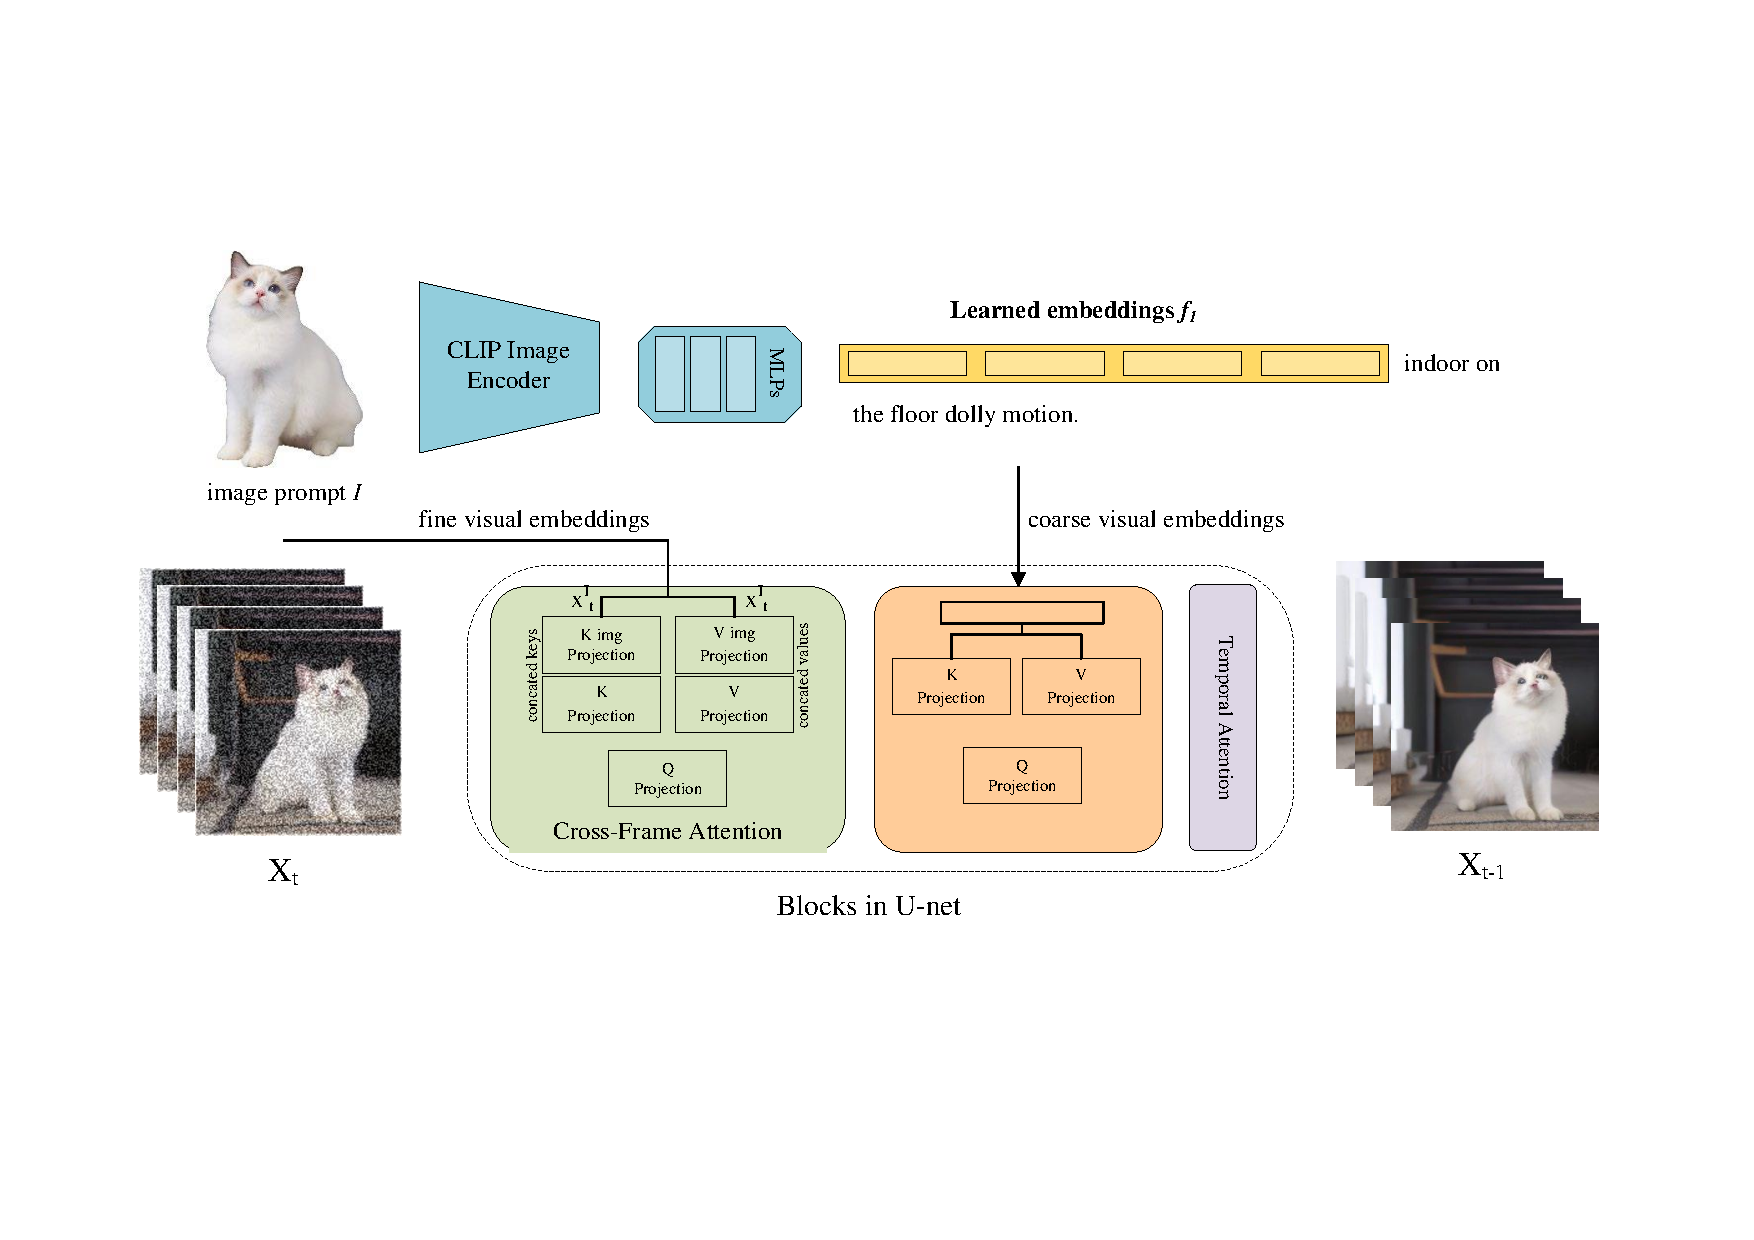
\includegraphics[width=\linewidth]{fig/main_framework.pdf}
    \caption{main\_framework}
\end{figure*}

Our proposed method aims at generating videos from an image prompt I and a text prompt T. As shown in \hyperref[main_framework]{Fig 1}, we use the image prompt specifies the appearance of the subject, which is fed into in two levels. First, we fed into a pretrained CLIP Image encoder to extract visual features. The encoder is composed of several MLP layers and is trained to map visual features into the space of text embeddings. After we obtain the embedding $f_I$, we insert them into text embedding, which is extracted by feeding text prompt $T$ into CLIP text encoder. In order to refine the details, we inject image prompt $I$ into the cross-frame attention module in the pretrained video diffusion model. Specifically, we incorporate the latent representation $x_t^I$ of the image prompt $I$ into the cross-frame attention mechanism. This approach integrates multi-scale visual details along with spatial information into the computation of attention maps, enhancing the preservation of visual characteristics. The image prompt is utilized in two complementary ways, operating in a coarse-to-fine manner: the encoder supplies coarse visual embeddings of the image prompt, while the attention injection introduces fine-grained visual embeddings.

\subsection{Coarse Visual Embeddings via Image Encoder}
Given an image prompt \(I\) and a text prompt \(T\), the generated video should align with both visual and textual elements. Inspired by previous image-based customization methods, we propose to encode the visual information of image prompts using an image encoder. The image prompt provides the visual characteristics of the desired subject in the video, while the text prompt contributes complementary information. The extracted visual embeddings are combined with text embeddings to form the final embeddings used in the cross-attention module.

Specifically, we utilize a pretrained CLIP image encoder to extract the visual features \(f_V\) from the image prompt \(I\). Since there is a discrepancy between CLIP image and text embeddings, \(f_V\) is mapped into the text embedding space using MLP layers \(F(\cdot)\), resulting in the final embedding \(f_I\) for the image prompt:

\[f_V = \text{CLIP}_I(I), \quad f_I = F(f_V)\]

The text prompt \(T\) is processed by the CLIP text encoder to extract text embeddings \(f_T\):

\[f_T = [f_T^0, f_T^1, \dots, f_T^k, \dots]\]

To integrate \(f_I\) and \(f_T\) for diffusion model conditioning, we replace the word embedding of the target subject in the text prompt with \(f_I\), resulting in the final text condition \(c_T\):

\[c_T = [f_T^0, f_T^1, \dots, f_T^{k-1}, f_I, f_T^{k+n}, \dots]\]

During training, the parameters of the CLIP image encoder are fixed, and the MLP layers are optimized. Additionally, we finetune the \(K\) and \(V\) projection layers in the cross-attention module to accommodate the composed embeddings \(c_T\).

\subsection{Fine Visual Embeddings via Attention Injection}
While the image encoder provides coarse visual embeddings, its high-level flattened representation may result in the loss of fine-grained visual details. To address this, we propose injecting the image prompt into the cross-frame attention module of the text-to-video model, allowing the model to directly incorporate detailed visual cues from the image prompt into the synthesized frames.

The image prompt is first passed through the VAE of Stable Diffusion to obtain its latent representation \(x_I\). Since video generation starts from noise, the latent representation needs to align with the intermediate states by adding noise:

\[x_I^t = \sqrt{\alpha_t}x_I^0 + \sqrt{1-\alpha_t}\epsilon\]

In cross-frame attention, we first update the values \(V_0\) of the first frame using the keys and values derived from the image prompt:

\[V_0^{\text{new}} = \text{softmax}\left(\frac{KQ_0^T}{\sqrt{d}}\right) \cdot V,\]
\[\quad K = [K_I, K_0], \quad V = [V_I, V_0]\]

Subsequently, the updated \(V_0^{\text{new}}\) is used to refine the remaining frames:

\[V_i^{\text{new}} = \text{softmax}\left(\frac{KQ_i^T}{\sqrt{d}}\right) \cdot V,\]
\[\quad K = [K_0, K_{i-1}], \quad V = [V_0^{\text{new}}, V_{i-1}]\]

To refine details further, we inject multi-scale latent representations of the image prompt into different cross-frame attention layers, using resolutions corresponding to different stages of the U-Net.

\subsection{Coarse-to-Fine Training Strategy}
The visual details of the image prompt are incorporated into the generated results in two stages: coarse visual embeddings via the image encoder and fine visual embeddings via attention injection. We propose a coarse-to-fine training strategy: first, the image encoder is trained to produce coarse embeddings, and then the attention injection module is trained to refine details.

As demonstrated in the ablation study, training both modules simultaneously causes the attention injection module to dominate, resulting in the image encoder learning ineffective representations. This leads to poor results during inference, as the coarse embeddings lack meaningful information to guide the attention injection module. Therefore, a sequential training strategy is essential to ensure the consistency and detail preservation in the synthesized video frames.

\subsection{Position encoding}
Position encoding is essential in transformer models to provide information about the order or position of input data. In our method, which involves generating videos from image and text prompts, position encoding helps capture both spatial and temporal relationships.

We utilize sine-cosine positional encodings, a common choice due to their ability to represent relative positions effectively. The standard formula is:

\[PE_{pos, 2i} = \sin\left( \frac{pos}{10000^{2i/d_{\text{model}}}} \right)\]\[
PE_{pos, 2i+1} = \cos\left( \frac{pos}{10000^{2i/d_{\text{model}}}} \right)\]

Where:
    \( PE \) is the positional encoding,
    \( pos \) is the position index,
    \( i \) is the dimension index,
    \( d_{\text{model}} \) is the embedding dimension.

For images, we extend this to 2D positions, encoding both width and height coordinates separately. For videos, we include temporal positional encodings to handle the sequence of frames.

In our cross-attention mechanism, position encodings are added to the query, key, and value embeddings to maintain coherence in spatial and temporal data. Additionally, for multi-scale latent representations, we scale the positional encodings to match the feature map sizes at different resolutions.

This approach ensures that our model effectively understands and utilizes the positional information in both spatial and temporal dimensions.

\subsection{LLM text prompt}
Large language models (LLMs) have demonstrated remarkable performance across a wide range of natural language tasks, showcasing their ability to understand and generate human language with remarkable accuracy and creativity. Their proficiency in handling complex linguistic structures and contextual nuances makes them invaluable tools for enhancing the quality of text prompts used in various applications, including image and video generation models. In these models, the text prompt serves as a critical guide, influencing the specificity and coherence of the generated content. The effectiveness of the prompt directly impacts the model's performance, and thus, improving prompt quality is essential for achieving desired outcomes.

Given the advantages of LLMs in generating detailed and contextually rich text, we have designed a prompt template \hyperref[LLM_text_prompt]{Table 1} that leverages their capabilities to refine and enhance the text prompts used in video generation models. This template is specifically crafted to capitalize on the LLM's strengths in understanding semantics and generating diverse descriptions, thereby producing more precise and effective prompts. By doing so, we aim to significantly improve the quality and fidelity of the generated videos, ensuring that they align closely with the intended visual content.

\begin{table}
    \caption{LLM text prompt.}
    \label{LLM_text_prompt}
    \begin{tabularx}{\linewidth}{X}
        \hline
            \ \ \ \ a man is playing guitar.\\
            \\
            \ \ \ \ Change the sentence above to something like this (add some facial changes, even if they are minor. Don't make the sentence too long):\\
            \\
            \ \ \ \ The video features a man standing next to an airplane, engaged in a conversation on his cell phone. he is wearing sunglasses and a black top, and he appears to be talking seriously. The airplane has a green stripe running along its side, and there is a large engine visible behind his. The man seems to be standing near the entrance of the airplane, possibly preparing to board or just having disembarked. The setting suggests that he might be at an airport or a private airfield. The overall atmosphere of the video is professional and focused, with the man's attire and the presence of the airplane indicating a business or travel context.\\
        \hline
    \end{tabularx}
\end{table}